%Simulation-based image generation
\subsection{Introduction}\label{ms:introduction}

To evaluate stereo-based 3D reconstruction algorithms, a large dataset of closely spaced image pairs with known relative camera poses is required.
That is difficult to obtain in practice, since jaw scans involve complex geometries and limited access paths. This section presents a simulation
environment that automatically generates such image datasets from pre-scanned jaw models, controlling the relative pose between adjacent images precisely.
The environment combines an UR5e collaborative robot \cite{universalrobots_ur5e_datasheet} with a custom camera tool modeled after the Sirona Omnicam\cite{dentsplysirona_cerec_ac_omnicam} scanner in PyBullet \cite{coumans2016pybullet}, using a modified IK solver for
arbitrary pose planning. High-quality images are rendered via a separate Blender instance that mirrors the simulation state, with customizable rendering settings \cite{blender_online_community}.
\subsection{Design Decisions and Implementation}\label{ms:design}

\subsubsection{Simulation with PyBullet}\label{ms:pybullet}

PyBullet \cite{coumans2016pybullet} serves as the physics and kinematics backbone. It loads the UR5e robot from a URDF description, provides forward and
inverse kinematics, collision detection and a GUI for inspection. All quantities are kept in SI units (metres) so that camera poses exported for the
reconstruction pipeline can be used without scaling. PyBullet was chosen because it is easy to use and well documented repo. The implementation builds on an
existing project repo\cite{ur5e_file_source}, that already provides a working UR5e model and basic motion planning, which was used as a starting point and extended with a custom ik solver
and integration into the whole program flow.

\subsubsection{Robot model and camera tool}\label{ms:ik}

An UR5e collaborative robot arm \cite{universalrobots_ur5e_datasheet} is modeled with six revolute joints, based on the afore mentioned repo\cite{ur5e_file_source}.
The custom camera tool is mounted on the tool flange and
consists of a scanner body plus left and right pinhole cameras with adjustable lateral offset, roll, field of view and near/far clipping. To reach the
dense waypoint sweeps around the jaw, the IK solver is used in a modified fashion: after the damped least-squares IK, a short iterative refinement with
the analytic Jacobian converges the end effector onto the desired tool-pose, and several collision-free seed configurations are tried when the first
result is in collision. Movement between waypoints is planned with the \emph{pybullet-planning} library (RRT with smoothing, fixed seed for
reproducibility) \cite{garrett2018pybulletplanning}.

\subsubsection{Realistic rendering with Blender}\label{ms:blender}

Physics-based rendering with PyBullet's built-in renderer is not photo-realistic enough for validating stereo reconstruction algorithms. Instead, a
separate Blender instance \cite{blender_online_community} builds the scene procedurally from the same URDF data and renders left/right image pairs with
the Cycles engine on the GPU. The Blender scene mirrors the simulation state over a TCP socket, so the rendered images correspond exactly to the
simulated camera poses.

\subsection{Code Structure and Workflows}\label{ms:structure}

\subsubsection{Component architecture}\label{ms:architecture}

The simulation is implemented as the Python package \code{ur5e\_bullet} (Figure~\ref{fig:ms-architecture}). \code{config.py} holds all parameters and is
standalone-loadable (no \code{pybullet} import, no relative imports), which allows the Blender scripts to import the same configuration in Blender's
own Python environment. \code{waypoints.py} supplies the parabola waypoints for each start position, \code{math\_utils.py} the quaternion
arithmetic, \code{sim.py} the simulation and IK/RRT planning, \code{camera.py} the camera poses in the jaw frame, \code{blender\_link.py} the TCP
client that mirrors joint states and coordinates rendering, and \code{demo.py} the interactive control loop. On the Blender side, \code{rig.py} builds
the scene and \code{mirror.py} provides the socket server and runs the Cycles rendering.

\begin{figure}[H]
    \centering
    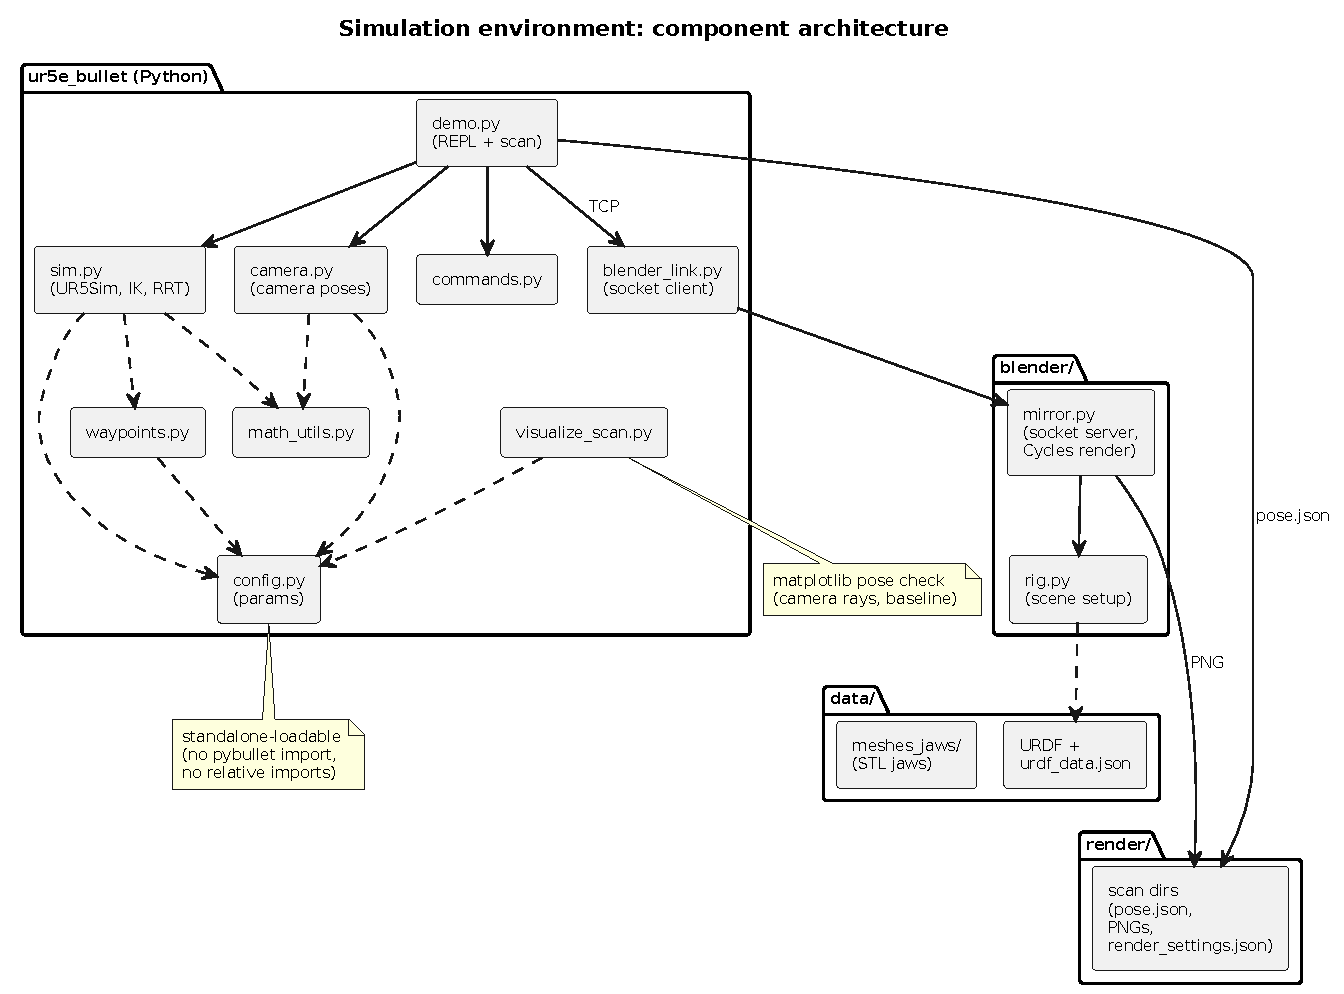
\includegraphics[width=\columnwidth]{assets/manuel/Architecture.pdf}
    \caption{Component architecture of the simulation environment. \code{config.py} is shared between the PyBullet pipeline and the Blender side.}
    \label{fig:ms-architecture}
\end{figure}

\subsubsection{Scan workflow}\label{ms:scan-workflow}

Starting from a user-selected start position with its jaw model loaded (STL geometry placed both in PyBullet and Blender), the scan sweep visits every
waypoint in order. At each waypoint the robot moves to the tool pose, the left/right camera poses are computed in the jaw frame and written to
\code{<n>\_pose.json}, and a render request for the left and right image is sent to Blender. Blender renders both views via Cycles on the GPU and
reports completion before the sweep advances. Figure~\ref{fig:ms-scan-workflow} shows the workflow; Figure~\ref{fig:ms-dataflow} details the message
and data flow for one waypoint together with the offline visualization step.

\begin{figure}[H]
    \centering
    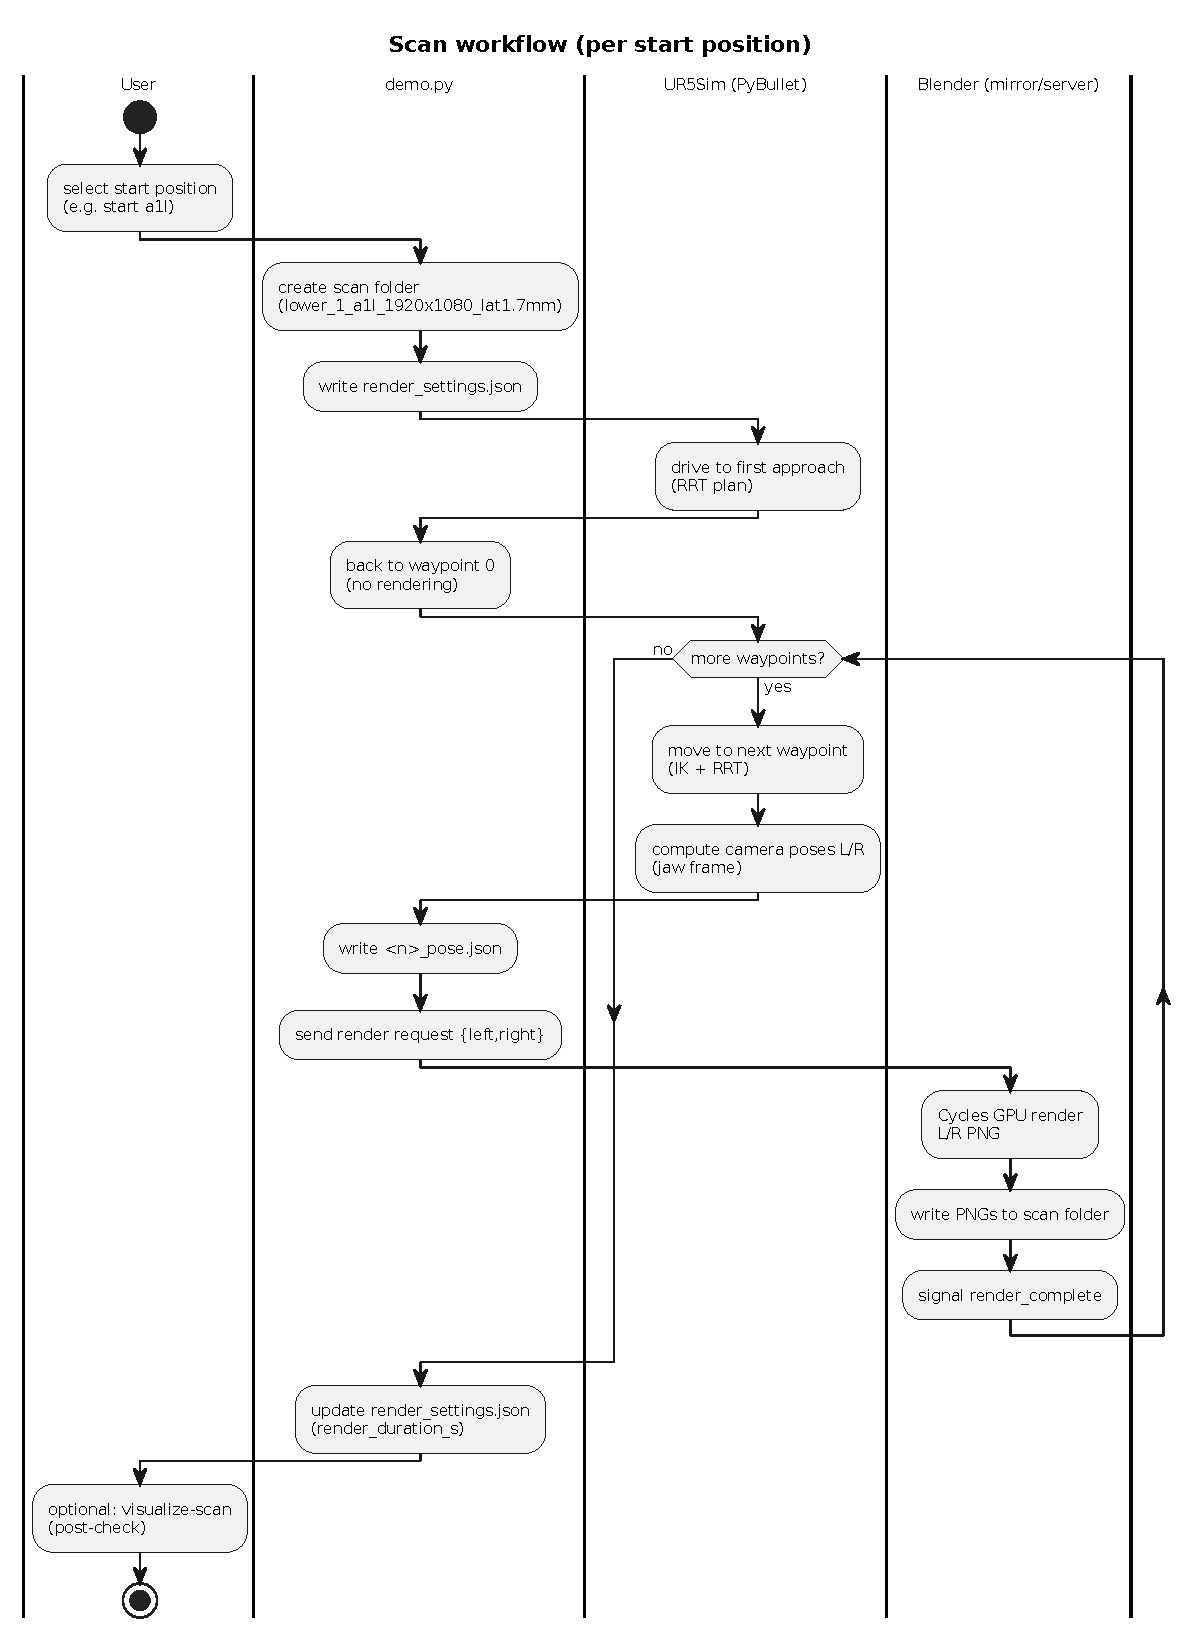
\includegraphics[width=\columnwidth]{assets/manuel/scan_workflow}
    \caption{Scan workflow for one start position. The sweep is driven by \code{demo.py}, executed by the PyBullet simulation and rendered by the Blender mirror.}
    \label{fig:ms-scan-workflow}
\end{figure}

\begin{figure}[H]
    \centering
    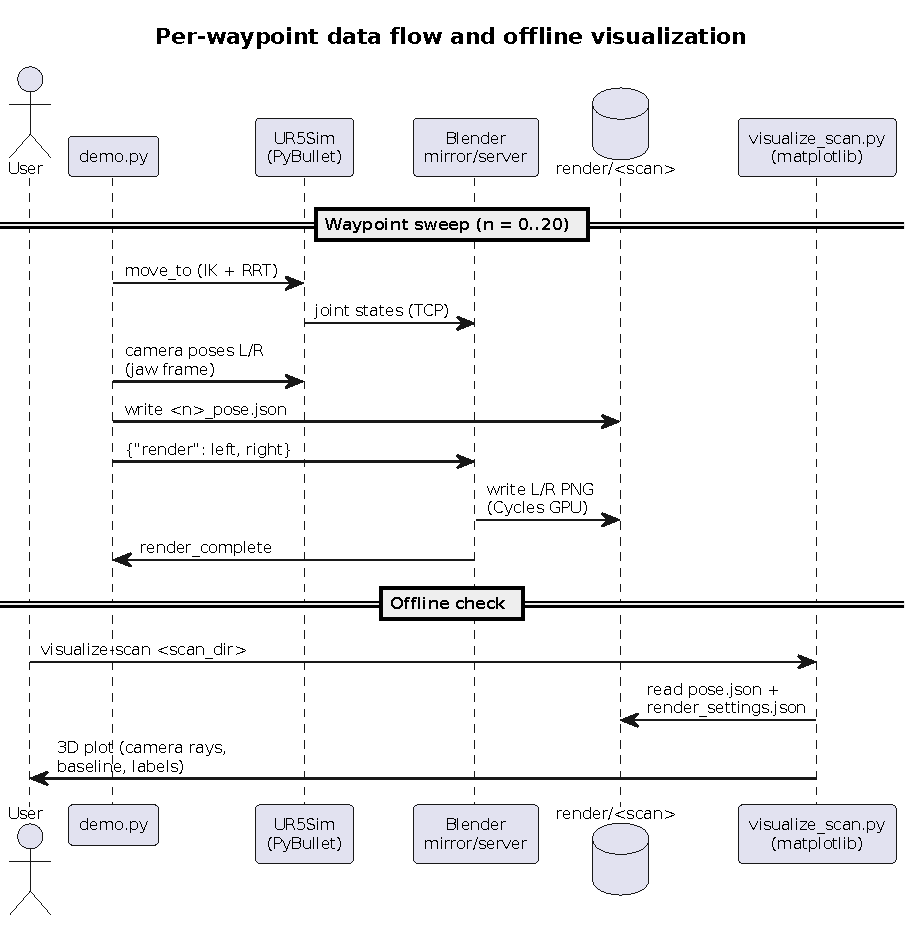
\includegraphics[width=\columnwidth]{assets/manuel/dataflow}
    \caption{Per-waypoint data flow and offline visualization of the exported camera poses.}
    \label{fig:ms-dataflow}
\end{figure}

\subsection{Usage}\label{ms:usage}

\subsubsection{Commands}\label{ms:commands}

The environment is started inside the project directory with the Poetry-managed dependencies:

\begin{itemize}[leftmargin=*]
    \item \code{poetry run ur5e} starts the PyBullet GUI, the Blender mirror and the interactive control loop.
    \item \code{start <name>} moves the arm to a start position and loads the jaw model (available: \code{a1l}, \code{a2l}, \code{aussen2}, \code{o1l}, \code{innen}).
    \item \code{scan [n]} drives all (or the first \code{n}) waypoints, saves the camera poses and renders the left/right images at each one.
    \item \code{scan-all <start1> [start2 ...]} runs \code{start} and a full \code{scan} for each given start position in sequence.
    \item \code{visualize-scan <scan\_dir|render/> [--out \ldots] [--ray-len m]} runs the offline pose check (Section~\ref{ms:visualization}).
\end{itemize}

\subsubsection{Configuration}\label{ms:config}

All parameters are collected in \code{src/ur5e\_bullet/config.py} and sorted by domain (paths, robot/kinematics, camera/sensor, rendering,
PyBullet GUI, visualization, jaw/material, Blender, scan positions). Central camera parameters used by both simulation and rendering are listed in
Table~\ref{tab:ms-camera-config}.

\begin{table}[H]
    \centering
    \small
    \caption{Central camera configuration parameters.}
    \begin{tabularx}{\columnwidth}{@{}>{\raggedright\arraybackslash}p{0.36\columnwidth} X@{}}
        \toprule
        \textbf{Parameter}                           & \textbf{Meaning}                                                                    \\
        \midrule
        \code{CAMERA_LATERAL_\newlineOFFSET}         & lateral offset of one camera from the scanner axis; \code{baseline\_m = 2 x offset} \\
        \code{CAMERA_FOV_DEG}, \code{CAMERA_LENS_MM} & horizontal field of view / lens focal length                                        \\
        \code{CAMERA_NEAR_M}, \code{CAMERA_FAR_M}    & near/far clipping planes of the pinhole camera                                      \\
        \code{CAMERA_ROLL_DEG}                       & roll of the camera rig around the viewing axis                                      \\
        \code{RENDER_W}, \code{RENDER_H}             & render resolution                                                                   \\
        \code{RENDER_ENGINE}, \code{RENDER_DEVICE}   & \code{CYCLES} on the \code{GPU}                                                     \\
        \code{START_POSITIONS}                       & start poses, approach poses and parabola waypoint generators                        \\
        \bottomrule
    \end{tabularx}
    \label{tab:ms-camera-config}
\end{table}

The \code{config.py} file is the only place to edit parameters; the values are forwarded into the live PyBullet session and, through the standalone
load, into Blender.

\subsubsection{Rendered dataset}\label{ms:results}

An example run with start position \code{a1l} produces the folder
\code{render/lower\_1\_a1l\_1920x1080\_lat1.7mm} containing 21 pose files
(\code{0\_pose.json} through \code{20\_pose.json}), 42 rendered PNGs (left/right per waypoint) and \code{render\_settings.json}. The pose file for each
waypoint stores \code{waypoint}, \code{label} and \code{camera\_left}/\code{camera\_right} with \code{position} and \code{quaternion} (x, y, z, w)
in the jaw coordinate frame. \code{render\_settings.json} stores the scan context (\code{start\_position}, jaw folder/type, jaw pose, render
resolution, engine/device, render duration) and the full reconstruction parameter block used by the stereo pipeline: \code{baseline\_m = 0.0034},
\code{camera\_fov\_deg = 87}, \code{camera\_lens\_mm $\approx$ 18.97}, \code{camera\_far\_m = 0.04}, \code{rectified = true},
\code{camera\_intrinsic} with \code{fx\_px = fy\_px = 1011.63}, \code{cx\_px = 960}, \code{cy\_px = 540} on a 36\,mm $\times$ 20.25\,mm sensor. A
second dataset with start position \code{o1l} is generated identically, which supports the stereo registration and model construction sections with
synthetic image pairs whose relative camera poses are known precisely.

\subsubsection{Visualization}\label{ms:visualization}

The offline pose visualization (\code{visualize-scan}) draws all camera rays (length = \code{camera\_far\_m}) from the \code{pose.json} files in the
jaw frame with \code{matplotlib}. As a \emph{positioning check} it shows the left (red) and right (blue) camera centers, the constant stereo baseline
(measured $\lvert \mathbf{L}-\mathbf{R}\rvert$, which should equal \code{baseline\_m}), the sweep order and the jaw bounding box. As an entry point
into the data work it provides the exact camera poses that feed the reconstruction pipeline, together with the ray geometry in orthographic
projection.

\subsubsection{Reconstruction reference}\label{ms:reconstruction}

The exported stereo pairs with known intrinsics and extrinsics are the input to the subsequent image acquisition and 3D reconstruction section. The
rectified left/right pairs enable standard stereo matching (e.g.\ SGM \cite{hirschmuller_stereo_2008} or learned methods such as IGEV-Stereo
\cite{xu_iterative_2023}) followed by point triangulation with the stated baseline; the \code{camera\_far\_m} value bounds the penetration of the
viewing rays into the jaw surface and can be used as a near-plane limit when triangulating intra-oral geometry. All pose files together realize the
photo-granular pose ground-truth that is otherwise hard to obtain for real intra-oral scans.